\documentclass{article}
\usepackage{graphicx}
\usepackage[T2A]{fontenc}
\usepackage[a4paper, margin=25mm, left=20mm, top=25mm, right=20mm, bottom=20mm, head=20mm, nofoot] {geometry}
\usepackage[utf8]{inputenc}
\usepackage{array}
\usepackage[russian]{babel}
\usepackage{float}
\usepackage{pdfpages}


\title{Дизайн документ}
\author{Андриянов Арсений, Александрова Ксения, Левицкая Алиса, \\ Печалинова Богдана, Соболев Григорий}


\date{Ноябрь 2024}

\begin{document}
	
	\maketitle
	
	\tableofcontents
	
	\newpage
	\section{Введение}
	Дальнейшее содержание этого документа организовано по разделам, в которых приводится следующая информация:
	\begin{itemize}
		\item Раздел 2. Концепция. Данный раздел содержит основные сведения об игре, включая общее описание, жанр, целевую аудиторию, предпосылки создания и основные особенности игры, а также информацию о платформах, на которых она будет доступна.
		\item Раздел 3. Функциональная спецификация. Этот раздел детально описывает функциональные аспекты игры, такие как принципы игрового процесса, физическая модель, характеристики персонажа, элементы игры, искусственный интеллект, многопользовательский режим, интерфейс пользователя, графика и видео, звуки и музыка, а также описание уровней.
		\item Раздел 4. Контакты. Данный раздел содержит контактную информацию для связи с разработчиками или другими заинтересованными лицами.
	\end{itemize}
	
	\newpage
	\section{Концепция}
	
	\subsection{Введение}
	Игра сочетает элементы \textit{хоррора, приключений, ролевой игры и мистического сюрреализма с головоломками и пиксельной графикой}. Она предназначена для аудитории от \textbf{14 лет и старше}. Игроки погружаются в мрачный и серый мир повседневной жизни, где реальность переплетается с мистикой, и каждое решение приводит к новым последствиям. Проект отличается напряженной атмосферой, нелинейным сюжетом, стратегическими элементами и глубоким нарративом, затрагивающим социальные и психологические проблемы, что делает его привлекательным для фанатов инди-разработок и атмосферных хорроров.
	
	\subsection{Жанр и аудитория}    
	Жанр игры можно определить как \textit{хоррор-приключенческий} с элементами ролевой игры, мистического сюрреализма и пиксельной графикой с головоломками. Игрокам предстоит погрузиться в мрачный и серый мир повседневной жизни обычного человека рабочего класса, где они столкнутся с различными мистическими загадками и кошмарами, отражающими истинные страхи людей в современного мире. \\  
	
	Игра ориентирована на взрослую аудиторию, в основном от \textbf{14 
		лет и старше}, что обусловлено наличием напряженной атмосферы и хоррор-сцен, а также сложных тем, которые могут не подойти более юной аудитории. Кроме того, игра привлекает людей, интересующихся инди-разработками и атмосферными, завлекательными нарративами, а также теми, кто хочет исследовать социальные и психологические проблемы, волнующие почти каждого человека на ежедневной основе. \\
	
	\subsection{Основные особенности игры}
	
	\textit{Ключевая особенность} игры состоит в том, что игрок вводится в игру не диалогами и записками, а посредством визуальных, звуковых и геймплейных деталей. Основная игровая задача -- передать атмосферу и эмоции главного героя через мрачные сочетания тонов, напряженные звуки и относительно высокую сложность игры. Также почувствовать ответственность за исход игры позволяет возможность игрока повлиять на развитие сюжета своими действиями.\\
	
	\textit{Длительность} прохождения зависит от игрока: от его адаптированности к подобному жанру и выбора концовки. Прохождение займет у игрока от 2 до 5 часов.\\
	
	\subsection{Описание игры} 
	
	\textit{The Twilight World} -- это увлекательная приключенческая игра, где игроки погружаются в новый мир, исследуя загадочные земли и решая разнообразные головоломки. Игра предлагает уникальный сюжет, насыщенный интересными персонажами и захватывающими квестами.\\
	
	Сюжет игры развернётся вокруг обычного человека, внезапно оказавшегося в мрачном, мистическом мире, где реальность искажена, а привычные места превратились в опасные лабиринты. Его главная цель -- выбраться живым и понять, \textit{что} привело его сюда.   
	Сначала главный герой начнёт замечать странные события: шепоты из пустых комнат, движущиеся тени и непонятные символы. По мере продвижения он найдет подсказки и артефакты, которые помогут понять природу происходящего, но для этого потребуется внимательность и логическое мышление. Ему также предстоит встречаться с таинственными сущностями, которые могут либо помочь, \textit{либо сбить с пути}. \\
	
	Сюжет будет нелинейным -- игроку придётся принимать решения, от которых зависят финал и разгадывания главной тайны. Игра создаст напряжённую атмосферу, где каждый шаг может привести как к спасению, так и к гибели, а загадки реального мира переплетаются с мистикой. \\
	
	
	\newpage
	\subsection{Предпосылки создания}
	
	Идея игры основывается на растущей популярности проектов, сочетающих психологический хоррор и элементы головоломки. Атмосферные инди-хорроры популярны в наши дни, как и игры с сильным визуальным стилем и глубоким сюжетом. Существование игр, совмещающих подобные жанры (например, "Yuppie Psycho", "Rusty Lake", "Amanda The Adventurer") демонстрирует, что игроки ищут в хорроре не только адреналин, но и глубокую историю с атмосферой, способной погрузить их в мир загадок, тревог и интриг. Данная игра предлагает уникальное сочетание: исследование мрачного, но знакомого мира, где реальность переплетается с мистикой, а каждое решение приводит к новым последствиям. \\
	
	\textit{Тенденции рынка:} сейчас растет популярность инди-игр с акцентом на хоррор стиль и атмосферу. Различные платформы (Steam, Epic Games) активно поддерживают проекты, которые выделяются своей эстетикой и идеей. Чёрно-белая палитра, минимализм и мистические элементы уже доказали свою успешность, привлекая как нишевых фанатов, так и широкую аудиторию. Кроме того, наличие нелинейного сюжета и элементов стратегии позволяет привлечь не только поклонников хорроров, но и игроков, ищущих интеллектуальные вызовы и разветвления в сюжете.
	
	\textit{Лицензирование и оригинальность:} весь игровой контент создаётся с упором на креативность, чтобы предложить уникальный продукт. Сюжет, персонажи и механики полностью авторские. \\
	
	Игры ужасов ценны своей способностью вызывать глубокий страх, который сложно испытать в реальной жизни, а эффект напряжения и последующего расслабления приносит игроку положительные эмоции. Наша игра построена на постоянном ощущении напряжения и дискомфорта, а не на банальных драках, что делает ее более осмысленной и эмоционально насыщенной. Это не просто аттракцион, а возможность для игрока испытать сложные чувства, исследуя мир, где мистика и реальность переплетаются. Проект имеет право на жизнь благодаря оригинальности концепции, сочетанию захватывающего геймплея с визуальным искусством и востребованности подобных игр на рынке.
	
	\subsection{Платформа}
	
	\begin{table}[h!]
		\centering
		\renewcommand{\arraystretch}{1.5}
		\setlength{\tabcolsep}{8pt}
		\begin{tabular}{|p{0.25\textwidth}|p{0.3\textwidth}|p{0.3\textwidth}|}
			\hline
			\multicolumn{3}{|c|}{\textbf{Для Windows}} \\ \hline
			\textbf{Требования} & \textbf{Минимальные} & \textbf{Рекомендуемые} \\ \hline
			\textit{Операционная система} & Windows 7 & Windows 10 \\ \hline
			\textit{Процессор} & Quad-core Intel \newline или AMD processor & Intel Core i5 \\ \hline
			\textit{ОЗУ} & 2 GB & 4 GB \\ \hline
			\textit{CD-ROM привод} & Нет & Нет \\ \hline
			\textit{Свободное место на HDD} & 4 GB & 4 GB \\ \hline
			\textit{Видеокарта} & NVIDIA GeForce 9800 GT \newline или AMD Radeon HD 4870 & NVIDIA GeForce GTX 750 Ti \newline или AMD Radeon R7 260X \\ \hline
			\textit{Звуковая карта} & Совместимая с DirectX 9.0c & Совместимая с DirectX 12 \\ \hline
			\textit{Управление} & Клавиатура и мышь & Клавиатура, мышь, геймпад \\ \hline
		\end{tabular}
		\caption{Системные требования для Windows}
		\label{tab:system-requirements1}
	\end{table}
	
	\begin{table}[h!]
		\centering
		\renewcommand{\arraystretch}{1.5}
		\setlength{\tabcolsep}{8pt}
		\begin{tabular}{|l|c|c|}
			\hline
			\multicolumn{3}{|c|}{\textbf{Для macOS}} \\ \hline
			\textbf{Требования} & \textbf{Минимальные} & \textbf{Рекомендуемые} \\ \hline
			\textit{Операционная система} & macOS X 10.8 & macOS 13.0 Ventura \\ \hline
			\textit{Процессор} &  Intel Core 2 Duo & Apple M1 \\ \hline
			\textit{ОЗУ} & 2 GB & 2 GB \\ \hline
			\textit{CD-ROM привод} & Нет & Нет \\ \hline
			\textit{Свободное место на HDD} & 4 GB & 4 GB \\ \hline
			\textit{Видеокарта} & Intel(R) HD Graphics 520 & Dedicated GPU supporting OpenGL \\ \hline
			\textit{Звуковая карта} & Встроенная & Встроенная \\ \hline
			\textit{Управление} & Клавиатура и мышь & Клавиатура, мышь, геймпад \\ \hline
		\end{tabular}
		\caption{Системные требования для macOS}
		\label{tab:system-requirements2}
	\end{table}
	
	\newpage
	\section{Функциональная спецификация}
	
	\subsection{Принципы игры}
	
	\subsubsection{Суть игрового процесса}
	
	Игровой процесс нашей игры предлагает глубокое погружение в мрачный и загадочный мир, где каждая деталь имеет значение, а каждое действие влияет на дальнейшее развитие сюжета. Основной акцент сделан на исследовании напряженной атмосферы и задачах, требующих внимательности и логического мышления, которые держат игрока в постоянном напряжении и заставляют задумываться над каждым шагом. \\
	
	\textbf{Основные эелементы геймплея:}
	
	\textit{Исследование.} Игрок перемещается по запутанным локациям, полным загадок, потайных ходов и интерактивных объектов. Мир наполнен скрытыми символами, записками и странными предметами, которые раскрывают детали сюжета. Каждая локация предлагает новые интерактивные элементы, будь то тайный замок, головоломка или необычный механизм, который необходимо активировать. Игроку предстоит внимательно осматривать окружение, чтобы находить ключи, подсказки и предметы для выживания.
	
	\textit{Головоломки.} Каждая локация предполагает логические задачи, которые тесно связаны с сюжетом. Игроку предстоит разгадывать шифры и символы, связанные с мистической историей, искать спрятанные механизмы и активировать их в правильной последовательности, собирать фрагменты информации для решения глобальных загадок, которые раскрывают ключевые аспекты мира игры.
	
	\textit{Элементы выживания и стратегия.}  Игроку придется управлять ограниченными ресурсами, включая здоровье,  редкие предметы и уникальные инструменты, такие как шприц с зеленым ядом. Принятие решений играет ключевую роль, игрок будет задаваться вопросом: "Использовать найденный предмет сейчас или сохранить его для более опасного момента?". Некоторые выборы будут влиять на развитие сюжета, изменение взаимоотношений с персонажами и конечного исхода игры.
	
	\textit{Сюжетное погружение.} История раскрывается через взаимодействие с миром, встречи с NPC и изменения в окружении. Игрок будет исследовать как реальные, так и мистические элементы, постепенно узнавая больше о природе происходящего. Сюжет развивается нелинейно, предлагая разные концовки в зависимости от решений игрока. \\
	
	Игра предложит игроку уникальный опыт: не только хоррор для андреналина, но и интеллектуальное, эмоционально насыщенное приключение, где страх и тайна создают незабываемую атмосферу. Игрок будет в постоянном напряжении и испытывать чувство неизвестности, а также удовольствия от постепенного раскрытия сложной и мистической истории. \\
	
	\subsubsection{Ход игры и сюжет}
	
	В этом хорроре игрока ожидает уникальный опыт, сочетающий напряженную атмосферу, глубокую интригу и необычную динамику взаимодействия с миром. Геймплей строится на исследовании, принятии решений и постоянной борьбе с неизвестным, заставляя задуматься о своей роли в происходящем. История медленно раскрывает связь главного героя с потусторонними событиями, держит в состоянии постоянного саспенса и предлагает искать ответы на непростые вопросы.
	
	Сеанс игры начинается с минималистичного меню. На экране – приглушенные тени, едва заметное мерцание и тихий шепот, создающий ощущение тревоги. После выбора "новая игра" начинается вступительная сцена, погружающая в историю. \\
	
	\textbf{Ход игры:}
	
	\textit{Игра открывается с видения:} в таинственном, искаженном мире раздаются голоса. Неопределенные фигуры, похожие на тени с размытыми очертаниями лиц, спорят о судьбе человека. Одни видят в нем ключ для восстановления порядка, другие – угрозу. Их спор прерывается яркой вспышкой, и игрок оказывается в обыденном офисе. За рабочим столом  просыпается главный герой, окруженный привычной суетой рабочего дня, но с самого начала что-то кажется не так.
	
	\begin{figure}[h]
		\centering
		\begin{minipage}{0.45\textwidth}
			\centering
			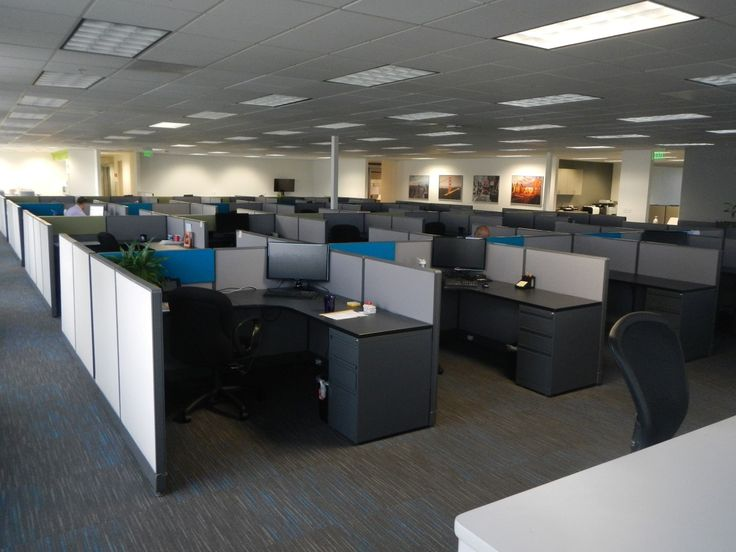
\includegraphics[width=\textwidth]{images/officeReference.jpg}
			\caption{Референс офиса}
			\label{fig:office}
		\end{minipage}
		\hfill
		\begin{minipage}{0.45\textwidth}
			\centering
			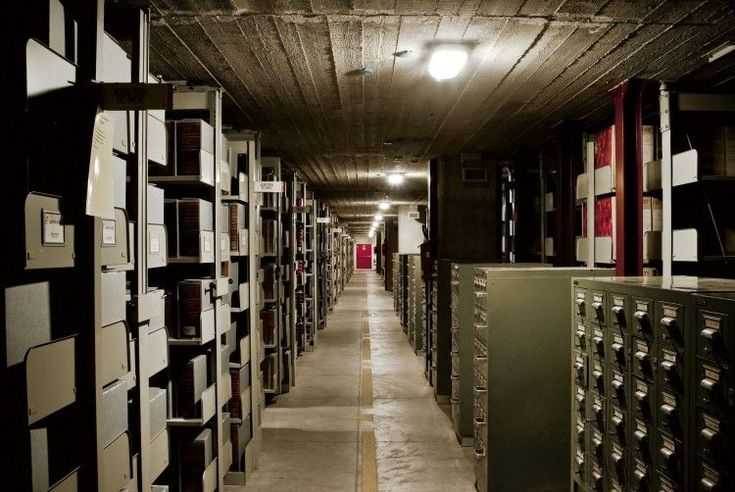
\includegraphics[width=\textwidth]{images/archive1.jpg}
			\caption{Референс архива}
			\label{fig:archive}
		\end{minipage}
	\end{figure}
	
	Игроку предоставляется возможность \textit{исследовать} офис. Задачи просты: взаимодействовать с предметами, читать записки, исследовать детали окружающего мира. Однако реальность постепенно становится всё более странной: часы идут в обратном направлении и растекаются, из мониторов доносится шепот, а лампы выключаются. Среди странностей – письмо, в котором намекается на скрытый архив. Игроку предстоит разгадать, как добраться до этой загадочной комнаты.
	
	\begin{figure}[H]
		\centering
		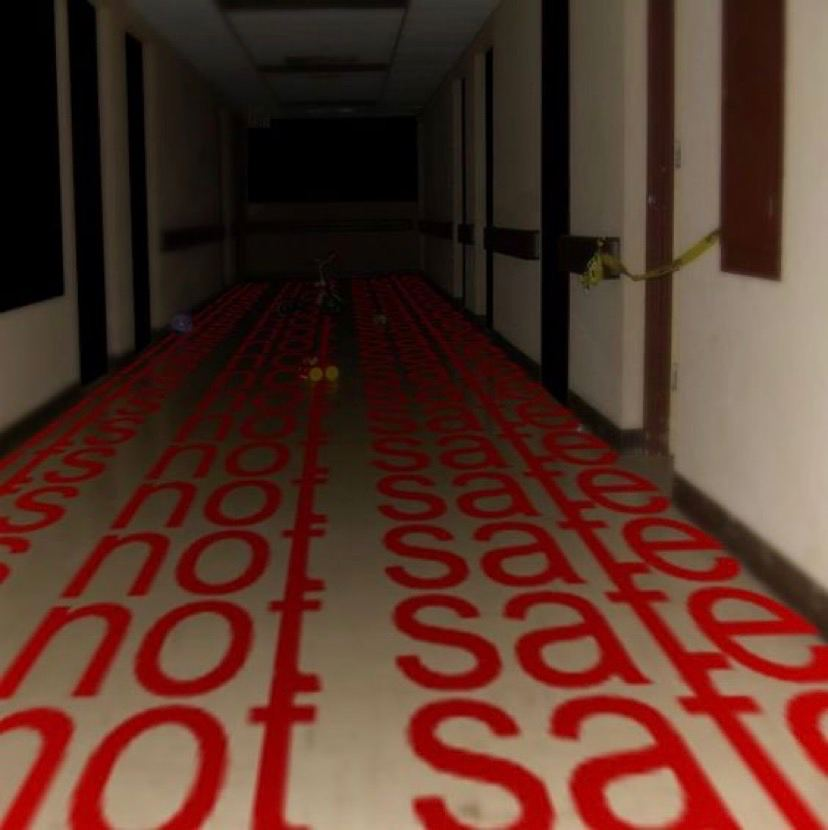
\includegraphics[width=0.4\textwidth]{images/pathtoarchive.jpg}
		\caption{Референс пути к архиву}
		\label{fig:path}
	\end{figure}
	
	\newpage
	\textit{Переход в потусторонний мир} происходит неожиданно. В архиве герой находит странный артефакт. Прикосновение вызывает вспышку, после которой мир меняется. Потусторонняя реальность полна искажений: тени становятся укрытием, свет – опасностью, а правила подчиняются неведомым силам. Здесь игроку придется адаптироваться к новым условиям и исследовать, как же связан герой с этим миром. На протяжении игры герой будет разгадывать загадки, исследовать переходы между мирами и взаимодействовать с таинственными предметами, чтобы понять причины хаоса и его влияние на обе реальности.
	
	\begin{figure}[h]
		\centering
		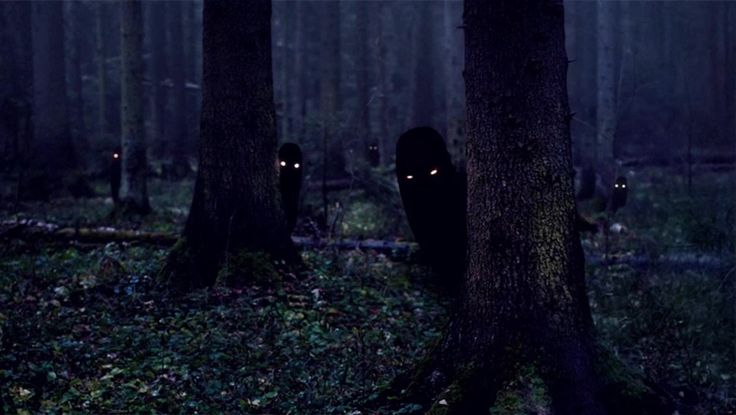
\includegraphics[width=0.45\textwidth]{images/otherworld.jpg}
		\caption{Референс потустороннего мира}
		\label{fig:otherworld}
	\end{figure}
	
	В процессе герой сталкивается с \textit{таинственными существами} – тенями, чьи маски отображают скрытые эмоции, и монстрами, собранными из фрагментов реальности. Одни из них предлагают помощь, другие ставят перед ним задачи или загадки. Но всегда остается вопрос: точны ли их намерения?
	
	\begin{figure}[h]
		\centering
		\begin{minipage}{0.45\textwidth}
			\centering
			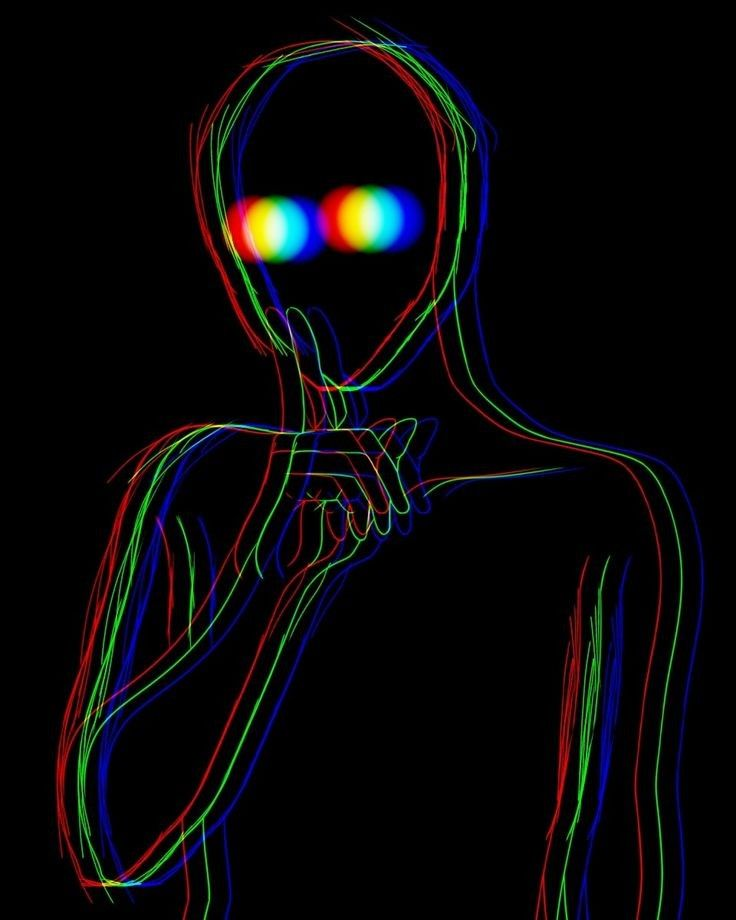
\includegraphics[width=\textwidth]{images/entity3.jpg}
			\caption{Референс таинственной сущности}
			\label{fig:entity1}
		\end{minipage}
		\hfill
		\begin{minipage}{0.4\textwidth}
			\centering
			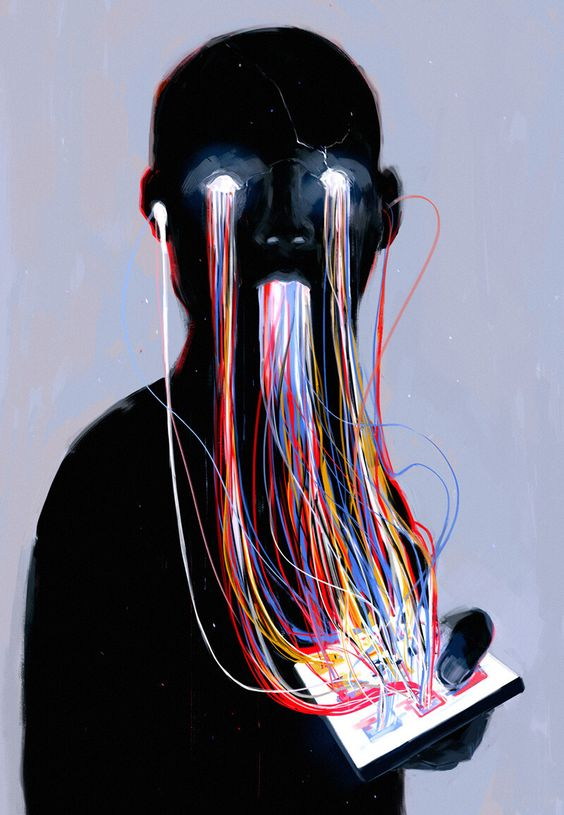
\includegraphics[width=\textwidth]{images/entity4.jpg}
			\caption{Референс таинственной сущности}
			\label{fig:entity2}
		\end{minipage}
	\end{figure}
	
	
	Сюжет разворачивается через загадки, диалоги и открытия. Игрок будет переходить между мирами, влияя на их состояние своими решениями. Офис и потусторонний мир становятся зеркалами, где действия героя оставляют след.
	
	\textit{Финал игры} держит в тайне истинные намерения всех сторон. Выборы игрока формируют концовку, но оставляют место для сомнений: правильно ли поступил герой? Почему коллеги избегают его взгляда? Что скрывают существа с другой стороны, называя его ключом? Кто из окружающих действительно хочет помочь, а кто скрывает истинные намерения? \\
	
	\newpage
	\textbf{Лор и история вселенной:}
	
	Потусторонний мир – это результат неудачных экспериментов по созданию порталов между человеческим сознанием и его тенью. Учёные хотели создать пространство чистого разума, но открыли двери в измерение, где человеческие страхи, желания и эмоции обретают форму.
	
	Этот мир наполнен существами, рожденными из подавленных эмоций. Одни стремятся уничтожить границы между реальностями, другие пытаются сохранить баланс. Герой оказывается втянут в эту историю, но вопрос остается открытым: случайно ли?
	
	Судьба мира зависит от игрока, но правда о герое может оказаться гораздо сложнее. Кто он в этой истории: спаситель, разрушитель или пешка в чужой игре?
	
	\subsection{Физическая модель}
	
	
	Физическая модель игрового мира является основой для создания реалистичного и увлекательного игрового опыта. Она определяет, как объекты взаимодействуют друг с другом, как игроки могут перемещаться по миру и как происходят боевые действия. Основные аспекты физической модели включают механизм перемещения, базовые законы динамики и систему расчетов для боевых действий.
	
	\textbf{Законы перемещения}
	
	\begin{itemize}
		\item \textbf{Ньютониевская динамика}: Все объекты подвержены законам механики. При движении объекта на него влияют силы (гравитация, трение, инерция).
		\item \textbf{Сила тяжести}: Все объекты в мире подвержены действию силы тяжести, что влияет на их поведение при прыжках, падении и перемещениях по наклонным поверхностям.
	\end{itemize}
	
	\textbf{Реализация перемещения в игре}
	\begin{itemize}
		\item \textbf{Контроль игрока}: Игроки управляют персонажами с помощью клавиатуры, которая реализуюет движения малых и больших перемещений (например, бег, прыжки, скольжение).
		\item \textbf{Физический движок}: Использовать физический движок (например, Unity Physics, Box2D или HavokPhysics) для обработки коллизий и законов движения в реальном времени.
		\item \textbf{Анимация}: Позаботиться о визуальной составляющей перемещения, обеспечив плавные анимации, синхронизированные с физическими действиями.
	\end{itemize}
	
	\textbf{Боевые действия}
	
	\begin{itemize}
		\item \textbf{Урон и сопротивление}: Урон от атаки рассчитывается исходя из силы удара и защиты цели. Также введена механика критических ударов.
		\item \textbf{Область действия}: Каждое оружие имеет радиус действия, который определяет область, в которой атака может быть успешной.
	\end{itemize}
	
	\textbf{Общие наиболее важные формулы}
	
	\begin{itemize}
		\item \textbf{Урон и сопротивление}
		\item \textbf{Сила удара}
	\end{itemize}
	
	\begin{figure}[h]
		\centering
		\begin{minipage}{0.45\textwidth}
			\centering
			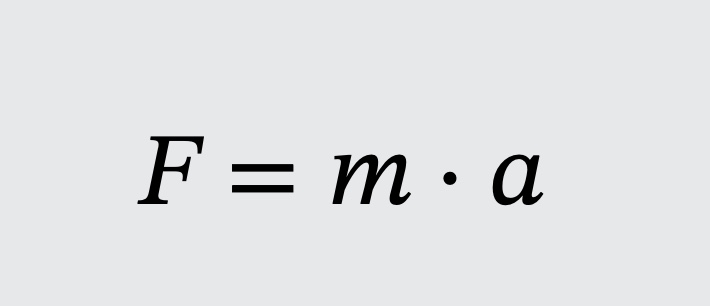
\includegraphics[width=\textwidth]{images/formula2.jpg}
			\caption{Формула модуля результирующего вектора силы, где F — сила, m — масса объекта, a — ускорение.}
			\label{fig:form2}
		\end{minipage}
		\hfill
		\begin{minipage}{0.45\textwidth}
			\centering
			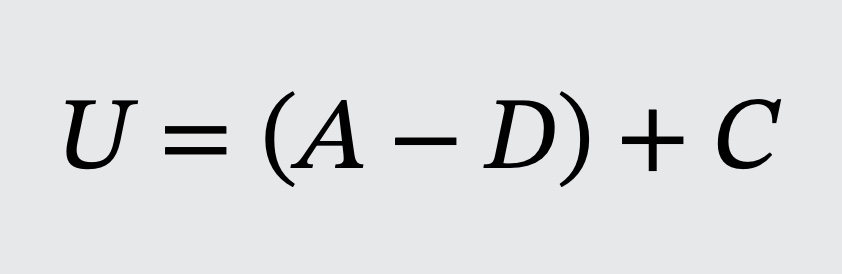
\includegraphics[width=\textwidth]{images/formula1.jpg}
			\caption{Формула урона от атаки, где U — урон, A — сила атаки, D — защита цели, C — дополнительный критический урон (если есть).}
			\label{fig:form1}
		\end{minipage}
	\end{figure}
	
	
	\newpage
	\subsection{Персонаж игрока}
	Главный герой — обычный офисный работник, который ведет рутинную жизнь, погруженный в повседневные заботы и обязанности. Однако его привычный мир резко меняется, когда он оказывается в мрачном и искаженном пространстве, полном загадок и опасностей. Внешне он ничем не примечателен: скромная офисная одежда и обыденная внешность делают его похожим на тысячи других людей. Тем не менее, за этой непримечательной оболочкой скрывается умение анализировать ситуацию и находить нестандартные решения.
	
	В новом мире герой сталкивается с множеством испытаний, требующих от него смелости и решительности. Он понимает, что для того чтобы выжить и найти путь обратно, ему нужно использовать свои способности для решения головоломок и разгадки тайн, окружающих его. Каждый шаг требует внимания и осторожности, а каждое открытие приближает его к пониманию причин своего появления в этом странном месте.
	
	Основная цель героя — выбраться из этого мрачного мира и понять причины своего появления здесь. Каждый его шаг и каждое решение могут существенно повлиять на развитие сюжета и финал истории. В процессе путешествия он будет сталкиваться с различными выборами, которые могут привести к неожиданным последствиям. 
	
	\begin{figure}[h]
		\centering
		
\includegraphics[width=0.45\textwidth]{images/main.jpg}
		\caption{Референс персонажа игрока}
		\label{fig:main}
	\end{figure}
	
	
	\subsection{Элементы игры}
	В данном разделе представлены ключевые элементы игры \textit{«The Twilight World»}, а также их функции, взаимодействие с игровым миром и игроками.
	
	\begin{itemize}
		\item \textbf{Предметы (Items):}  \\
		\textit{Назначение:} Предметы являются основным инструментом решения головоломок и исследования мира. Они могут быть как обычными объектами вроде ключей и фонариков, так и мистическими артефактами, обладающими особыми свойствами.  \\
		\textit{Влияние на игрового персонажа:} Некоторые предметы дают возможность открывать новые области карты, другие защищают героя от опасностей или позволяют видеть скрытые объекты.  \\
		\textbf{Параметры:}  \\
		\textit{Тип предмета:} Обычный, магический, редкий.  \\
		\textit{Свойства:} Свет, защита, исцеление, усиление интуиции.  \\
		\textit{Редкость:} Обычные, редкие, легендарные.  \\
		\textbf{Примеры предметов:}
		\begin{itemize}
			\item Фонарь: Позволяет освещать темные места и находить скрытые подсказки.
			\item Ключ: Открывает двери и сундуки.
			\item Амулет: Защищает от определенных видов угроз.
		\end{itemize}
		\begin{figure}[h]
			\centering
			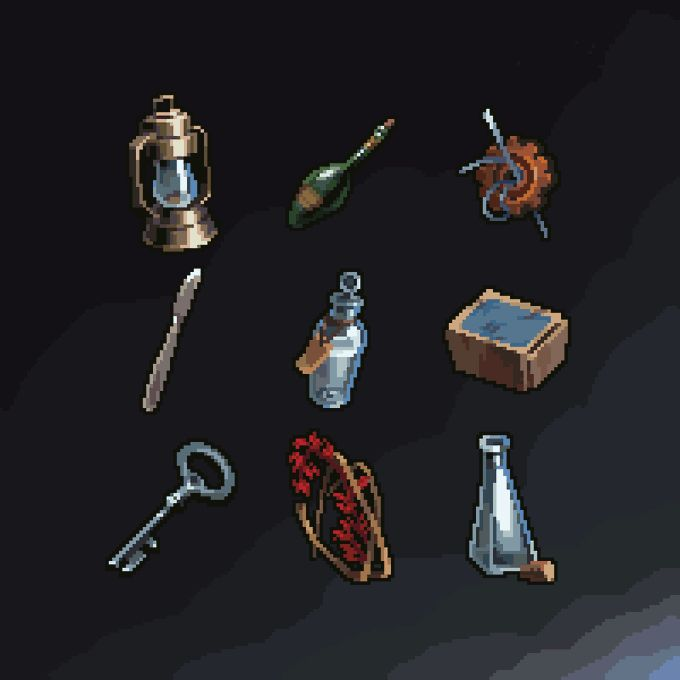
\includegraphics[width=0.45\textwidth]{images/items1.jpg}
			\caption{Референс предметов}
			\label{fig:items}
		\end{figure}
		\newpage
		
		\item \textbf{NPC и Персонажи:}  \\
		\textit{Назначение:} NPC играют важную роль в сюжете и помогают игроку продвигаться вперед через предоставление информации, заданий и решений головоломок.  \\
		\textit{Взаимодействие с игроком:} Игрок может общаться с NPC, чтобы получить информацию о мире, заданиях или головоломках. Некоторые NPC могут быть враждебными и представлять угрозу.  \\
		\textbf{Особенности:}  \\
		\textit{Личность:} Каждый NPC имеет свою уникальную личность и историю, которая раскрывается по мере прохождения игры.  \\
		\textit{Роль в сюжете:} Одни NPC будут союзниками, другие врагами, третьи нейтральны.  \\
		\textbf{Примеры персонажей:}
		\begin{itemize}
			\item Мэри: Старушка, живущая в заброшенном доме. Она знает много тайн об истории этого места и поможет вам найти важные ключи к разгадке.
			\item Тень: Таинственный персонаж, который будет преследовать вас на протяжении всей игры, создавая ощущение постоянного страха.
		\end{itemize}
		\begin{figure}[h]
			\centering
			\begin{minipage}{0.4\textwidth}
				\centering
				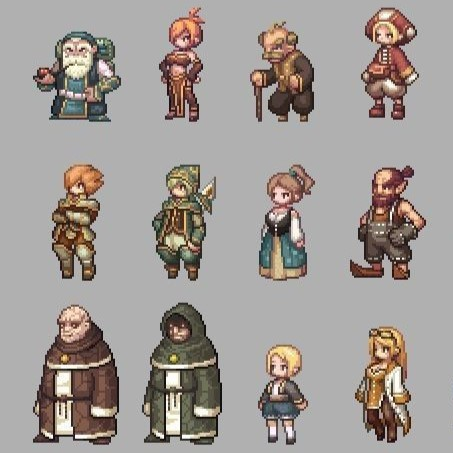
\includegraphics[width=\textwidth]{images/civilians.jpg}
				\caption{Референс мирных NPC}
				\label{fig:civilians}
			\end{minipage}
			\hfill
			\begin{minipage}{0.4\textwidth}
				\centering
				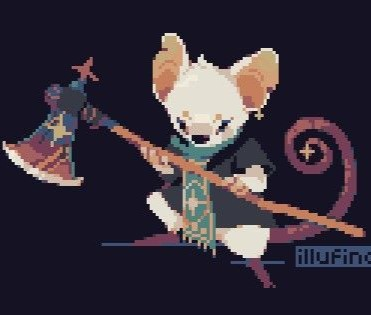
\includegraphics[width=\textwidth]{images/sage.jpg}
				\caption{Референс проводника}
				\label{fig:sage}
			\end{minipage}
		\end{figure}
		\begin{figure}[h]
			\centering
			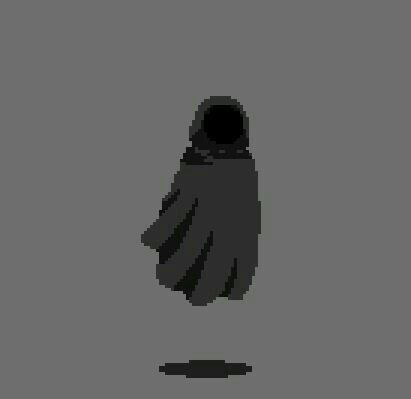
\includegraphics[width=0.45\textwidth]{images/shadow.jpg}
			\caption{Референс преследователя}
			\label{fig:shadow}
		\end{figure}
		\newpage
		
		\item \textbf{Головоломки:}  \\
		\textit{Назначение:} Головоломки являются основой геймплея. Они варьируются от простых задач до сложных логических загадок, требующих использования различных предметов и взаимодействия с окружающей средой.  \\
		\textit{Влияние на игровое развитие:} Решение головоломок открывает доступ к новым областям карты, помогает продвигаться по сюжету и получать ценные предметы.  \\
		\textbf{Типы головоломок:}  
		\begin{itemize}
			\item Простые (ключ-ящик).
			\item Логические (разгадывание шифров, кодов).
			\item Механические (управление механизмами, использование предметов).
			\item Тайминговые (реакция на события в реальном времени).
		\end{itemize}
		\textbf{Пример головоломки:}
		\begin{itemize}
			\item «Секретный проход»: Чтобы открыть потайную дверь, нужно правильно расставить символы на древнем алтаре, используя найденные подсказки.
		\end{itemize}
		
		
		\item \textbf{Оружие:}  \\
		\textit{Назначение:} В игре оружие используется не столько для уничтожения врагов, сколько для защиты и активации некоторых механизмов.  \\
		\textit{Использование:} Игроки должны использовать оружие стратегически, чтобы преодолеть препятствия и защитить себя от неожиданных атак.  \\
		\textbf{Виды оружия:}  
		\begin{itemize}
			\item Магическое: Например, амулеты, способные отпугивать злых духов.
			\item Механическое: Молот для разбивания преград, нож для разрезания веревок.
		\end{itemize}
		\begin{figure}[H]
			\begin{minipage}{0.4\textwidth}
				\centering
				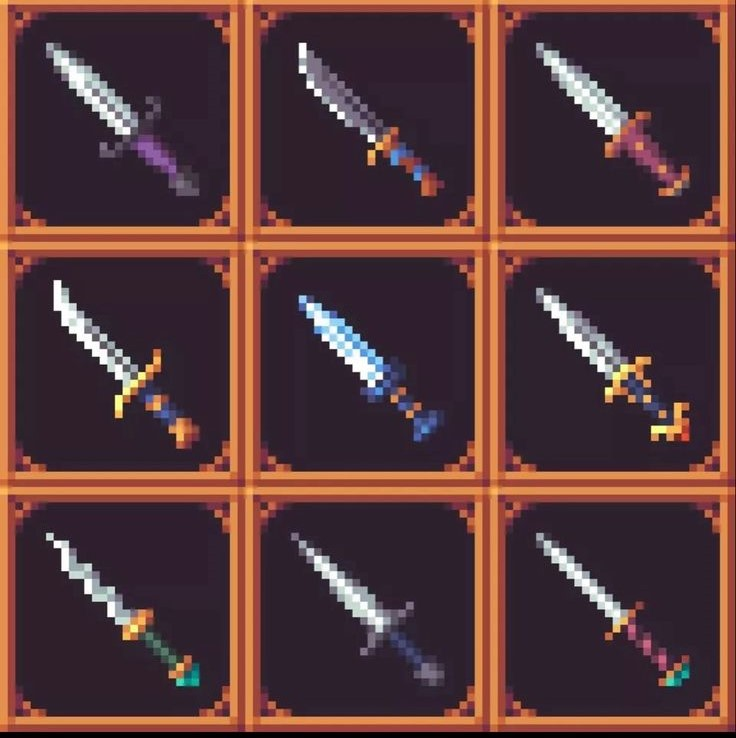
\includegraphics[width=\textwidth]{images/knives.jpg}
				\caption{Референс механического оружия}
				\label{fig:weapon1}
			\end{minipage}
			\hfill
			\begin{minipage}{0.4\textwidth}
				\centering
				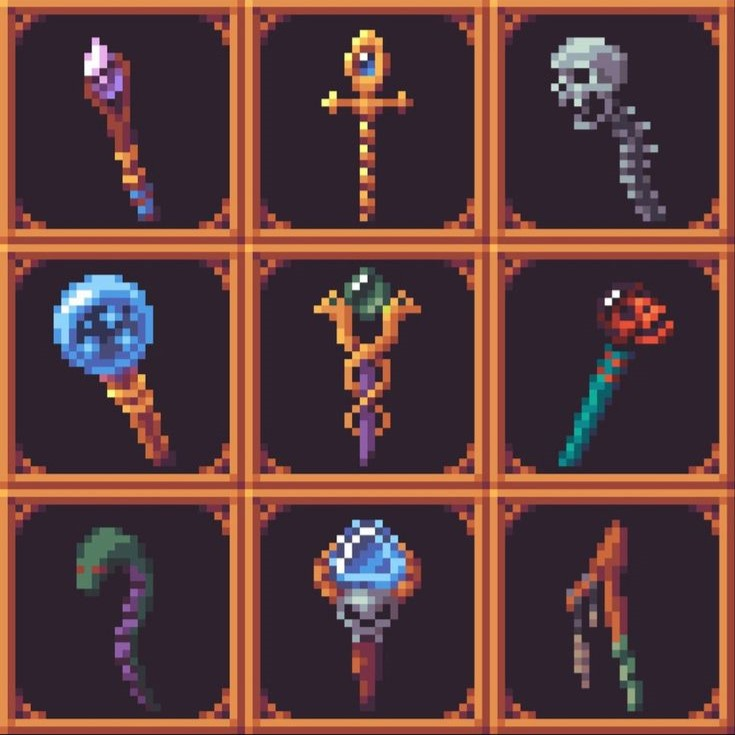
\includegraphics[width=\textwidth]{images/magical.jpg}
				\caption{Референс магического оружия}
				\label{fig:weapon2}
			\end{minipage}
		\end{figure}

		
		\item \textbf{Транспортные средства:}  \\
		\textit{Назначение:} Для перемещения между различными локациями в мире игры.  \\
		\textit{Функции:} Быстрое перемещение, доступ к труднодоступным местам.  \\
		\textbf{Примеры транспортных средств:}
		\begin{itemize}
			\item Старый автомобиль, который можно починить.
			\item Лодка для переправы через реку.
		\end{itemize}
		\begin{figure}[h]
			\begin{minipage}{0.4\textwidth}
				\centering
				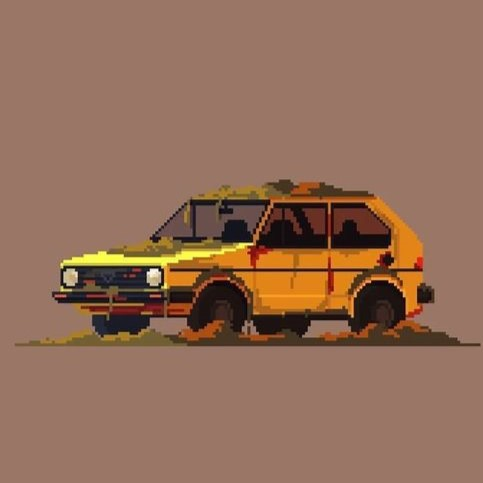
\includegraphics[width=\textwidth]{images/car.jpg}
				\caption{Референс транспорта}
				\label{fig:transport1}
			\end{minipage} % Закрывающая скобка добавлена здесь
			\hfill
			\begin{minipage}{0.4\textwidth}
				\centering
				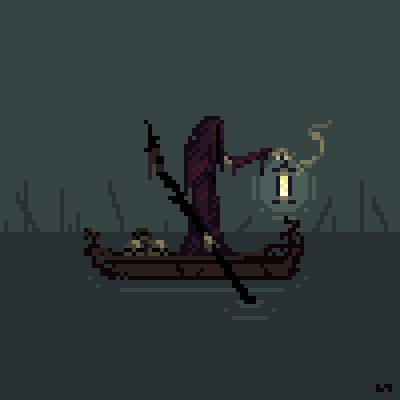
\includegraphics[width=\textwidth]{images/ship.jpg}
				\caption{Референс транспорта}
				\label{fig:transport2}
			\end{minipage}
		\end{figure}
		
		\item \textbf{Карты:}  \\
		\textit{Назначение:} Помогают ориентироваться в мире игры, показывают местоположение ключевых объектов и подсказывают пути решения головоломок.  \\
		\textbf{Типы карт:}  
		\begin{itemize}
			\item Общая карта мира.
			\item Карта конкретной локации.
			\item Секретная карта, показывающая скрытые проходы.
		\end{itemize}
	\end{itemize}
	
	Эти элементы составляют основу игрового процесса и создают атмосферу таинственности и напряжения, характерные для жанра хоррора.
	
	\subsection{«Искусственный интеллект»}
	В игре \textit{«The Twilight World»} искусственный интеллект (AI) выполняет важную роль в формировании атмосферы и взаимодействий в игровом процессе. Рассмотрим, как именно это происходит.\\
	
	\textbf{Основные принципы, характеризующие AI в игре:}
	\begin{itemize}
		\item\textit{Поведенческая адаптация:} AI в игре реагирует на действия игрока и меняет свое поведение в зависимости от выбора игрока, создавая ощущение динамичного мира.
		
		\item\textit{Интерактивные NPC:} Персонажи с AI имеют разнообразные модели поведения. Некоторые из них могут быть дружелюбными и предоставлять полезную информацию, в то время как другие могут проявлять агрессивность или недовольство, что создает напряжение.
		
		\item\textit{Загадки и задачи:} AI управляет элементами головоломок и задач, которые игрок должен решить для продвижения по сюжету. Это может включать в себя создание ловушек или препятствий, которые заставляют игрока думать и принимать решения.
		
		\item\textit{Управление атмосферой:} AI также отвечает за поддержание общего настроения игры, демонстрируя элементы страх или напряжение в взаимодействии с играющими. Это помогает погрузить игрока в атмосферу офисного триллера.
		
		\item\textit{Динамичные сценарии:} Ситуации и взаимодействия, зависящие от поведения AI, могут развиваться по-разному в зависимости от ходов игрока, что добавляет элемент непредсказуемости и разнообразия в игровой процесс.
	\end{itemize}
	AI в \textit{«The Twilight World»} не представлен как абсолютный разум, а скорее как инструмент, помогающий создать уникальный, интерактивный опыт, который заставляет игрока чувствовать себя частью живого мира, полным загадок и угроз.\\
	
	\subsection{Интерфейс пользователя}
	
	\subsubsection{Блок-схема}
	
	Привиденные ниже блок-схемы отражают взаимодействие игрока с механиками и этапами прохождения. Акцент сделан на динамическом погружении в сюжет. Навигация по игровым механикам и их взаимосвязь показаны через последовательность действий и событий.
	
	\newpage
	\begin{figure}[h!]
		\centering
		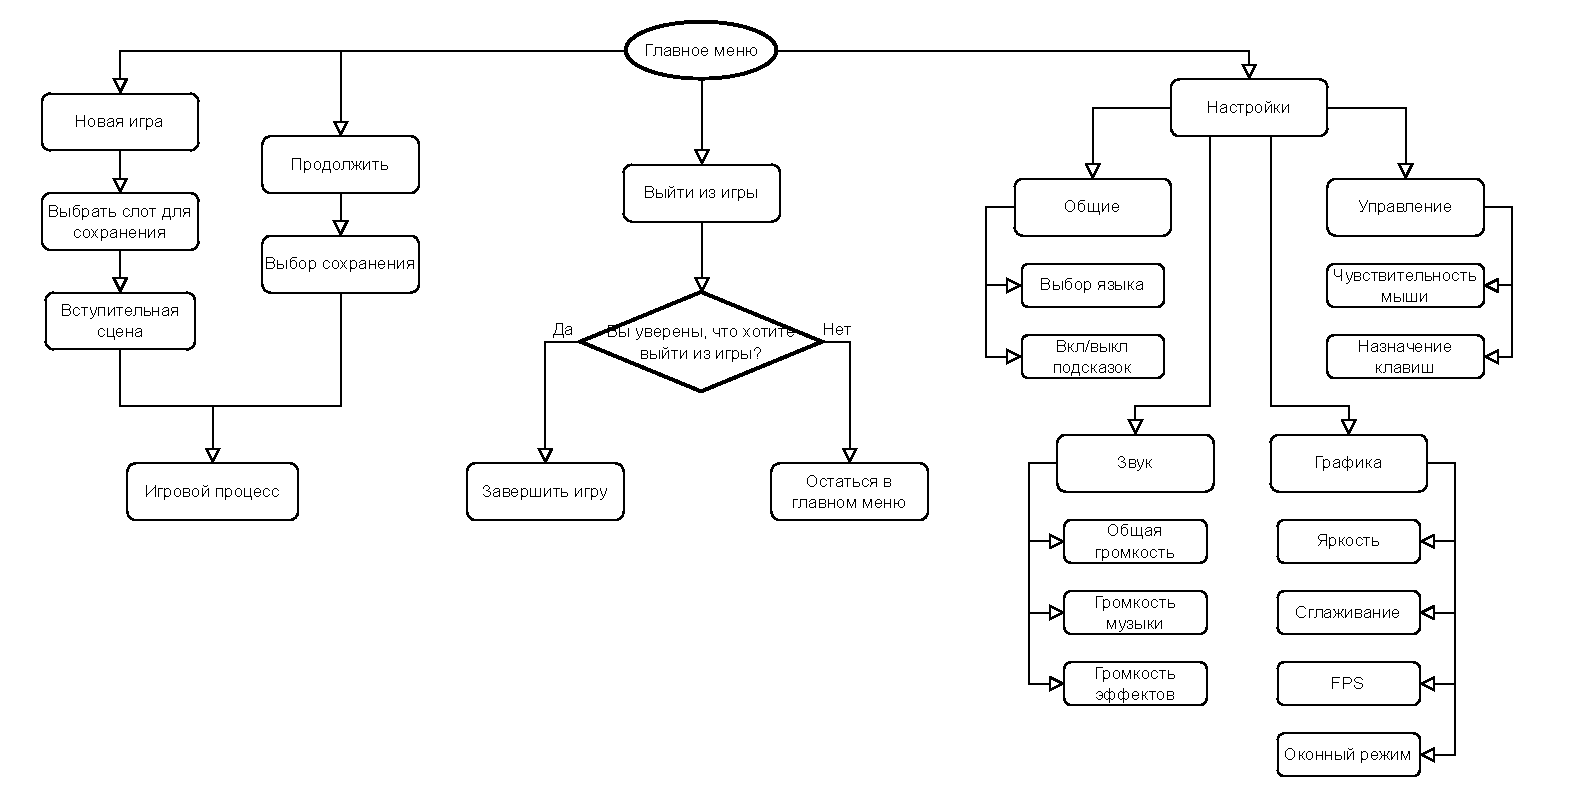
\includegraphics[width=\textwidth]{images/блоксхема1-2.pdf} 
		\caption{Схема навигации по меню игрового интерфейса}
		\label{fig:pdf-example}
	\end{figure}
	
	\begin{figure}[h!]
		\centering
		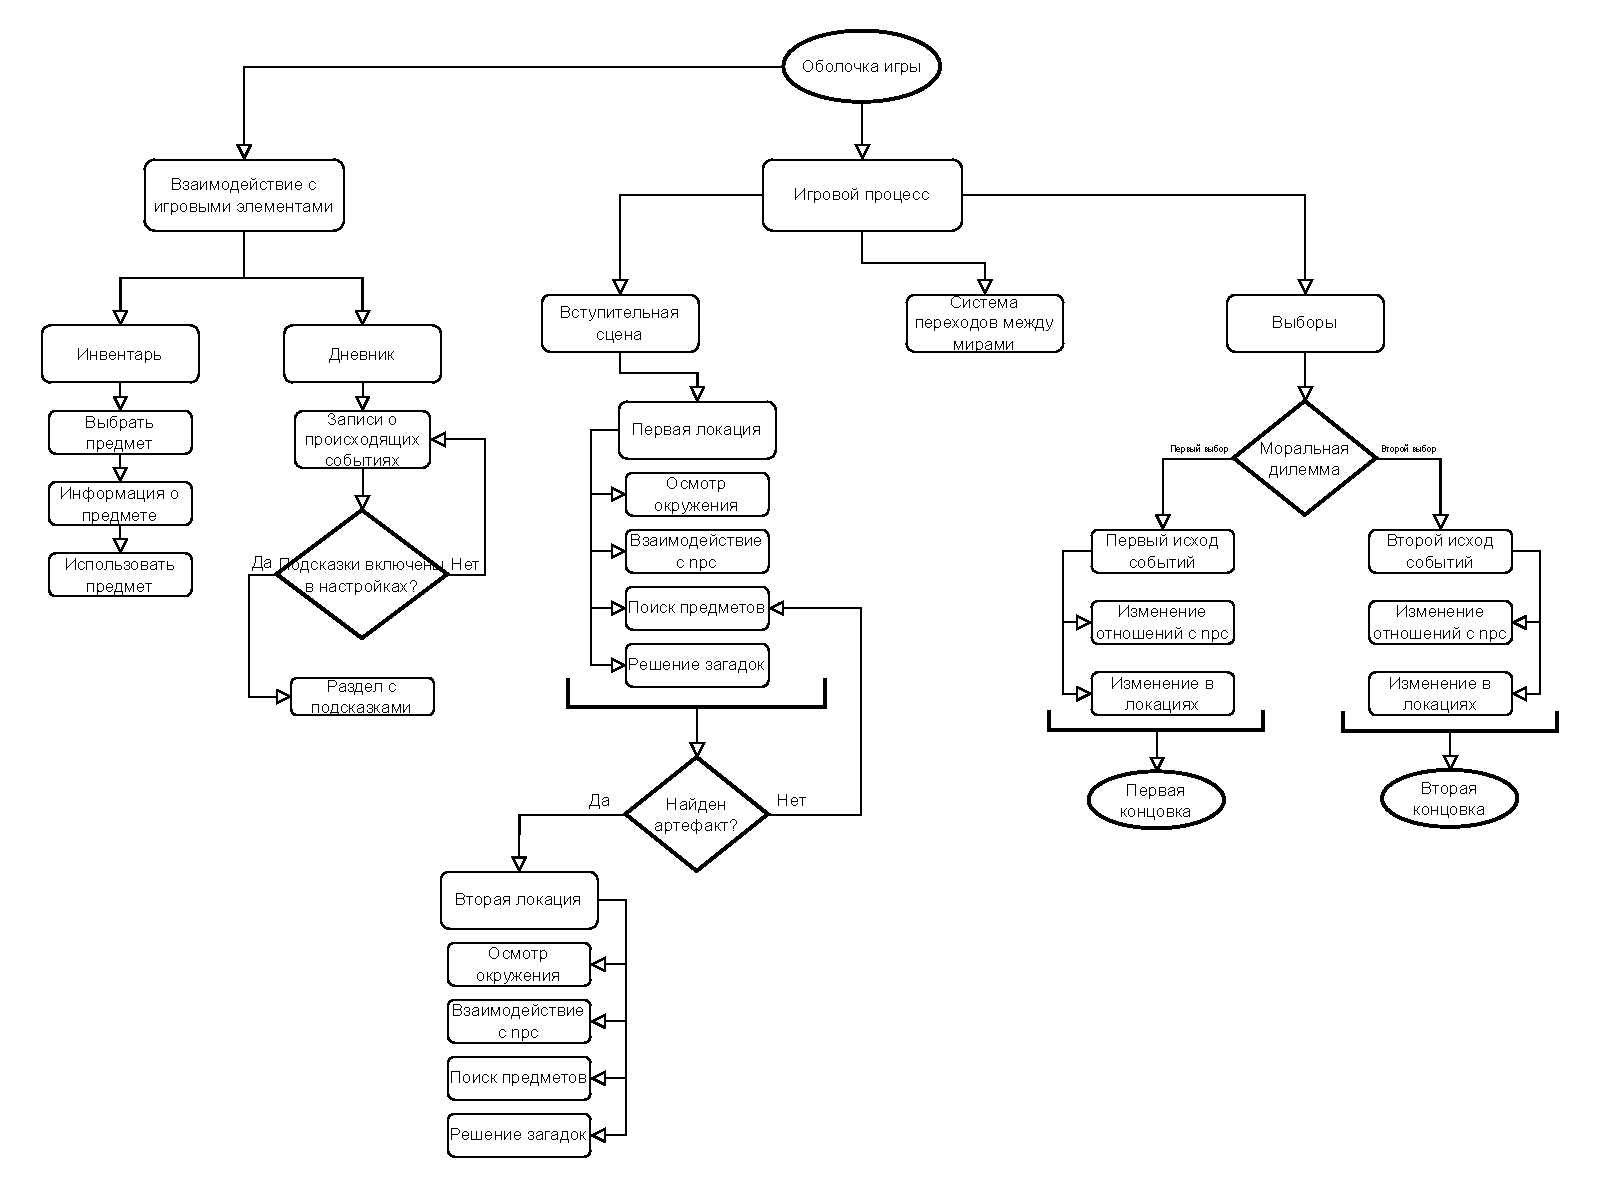
\includegraphics[width=\textwidth]{images/блоксхема2-3.pdf}
		\caption{Схема оболочки игры}
		\label{fig:pdf-example2}
	\end{figure}
	
	\newpage
	\subsubsection{Функциональное описание и управление}

	\paragraph{Главное меню.}
    \begin{itemize}
        \item \textbf{Функциональность:} Доступ к основным разделам игры (игра, настройки, выход).
        \item \textbf{Управление:} Навигация осуществляется мышью или клавишами стрелок. Выбор подтверждается нажатием клавиши Enter или левой кнопки мыши.
    \end{itemize}
    
    \paragraph{Игровой экран.}
    \begin{itemize}
        \item \textbf{Функциональность:} Отображение параметров персонажа (здоровье, мана), карты и действий игрока.
        \item \textbf{Управление:} 
        \begin{itemize}
            \item Движение — клавиши WASD.
            \item Атака — левая кнопка мыши.
            \item Меню паузы — клавиша Esc.
        \end{itemize}
    \end{itemize}
    
    \paragraph{Экран инвентаря.}
    \begin{itemize}
        \item \textbf{Функциональность:} Просмотр и управление предметами.
        \item \textbf{Управление:} Навигация — стрелки клавиатуры или мышь. Использование предмета — клавиша E.
    \end{itemize}
    
	
	\subsubsection{Объекты интерфейса пользователя}
	
	\subsection{Графика и видео}
	\subsubsection{Общее описание}
    Проект выполнен в 2D пиксельной графике, что придает ему уникальный визуальный стиль, характерный для инди-игр. Пиксельная эстетика создает атмосферу ностальгии и одновременно передает мрачные и сюрреалистические элементы игрового мира.
    
    Сочетание элементов хоррора, приключений, ролевых игр и мистического сюрреализма формирует атмосферу, которая является мрачной и угнетающей. Преобладание черно-белой палитры усиливает чувство тревоги и неопределенности, погружая игроков в серый мир повседневной жизни рабочего класса, где каждое решение имеет последствия. Мистические элементы и головоломки добавляют глубины, а минималистичный стиль помогает сосредоточиться на нарративе и эмоциональных переживаниях главного героя.
    
    Ориентированность на взрослую аудиторию от 14 лет и старше обусловлена наличием сложных тем, напряженных сцен и элементов хоррора, которые могут быть неуместны для более юной аудитории. Ключевой особенностью проекта является отсутствие традиционных диалогов и записок для передачи сюжета; вместо этого игроки погружаются в мир через визуальные и звуковые детали, что усиливает эмоциональную нагрузку. Нелинейный сюжет и возможность влиять на развитие истории делают игру привлекательной не только для поклонников хорроров, но и для тех, кто ищет интеллектуальные вызовы и разветвленные нарративы.
   
	\subsubsection{Двумерная графика и анимация}
	
	\subsubsection{Трехмерная графика и анимация}
	
	\subsubsection{Анимационные вставки}
	
	\subsection{Звуки и музыка}
	
	\subsubsection{Общее описание}
	
	\subsubsection{Звук и звуковые эффекты}
	
	\subsubsection{Музыка}
	
	\subsection{Описание уровней}
	
	\subsubsection{Общее описание дизайна уровней}
	
	\subsubsection{Диаграмма взаимного расположения уровней}
	
	\subsubsection{График введения новых объектов}
	
	\newpage
	\section{Контакты}
	
	\newpage
	
\end{document}
